\subsection{Git}
Git е система за контрол на версиите, която проследява промените във всеки
набор от компютърни файлове. Обикновено се използва за координиране на работата
между програмистите, които съвместно разработват изходния код по време на
разработката на софтуер. Целите на системата включват скорост, цялост на
данните и поддръжка за разпределени, нелинейни работни потоци (хиляди паралелни
клонове, работещи на различни системи).

Git първоначално е създаден от Линус Торвалдс, през 2005 година за разработване
на Linux ядрото, като инструмен за други разработчици, които допринасят за
първоначалното му развитие. От 2005 година Джуино Хамано е основният
разработчик. Както при повечето други разпределени системи за контрол на
версиите и за разлика от повечето системи клиент-сървър, всяка Git директория
на всеки компютър е пълноценно хранилище с пълна история и пълни възможности за
проследяване на версиите, независимо от достъпа до мрежата или централен
сървър. Git е безплатен софтуер с отворен код, разпространяван само под лиценз
GPL-2.0. \cite{git_wikipedia}

Git е конзолно приложение, но съсществуват и приложения с графичен интерфейс.
Най-често използваното такова е GitHub Desktop. Това приложение ни дава
възможност да управляваме разработката на проекта, да създаваме потребителски
истории и тяхното управление. [Фигура \ref{fig:github-desktop}]
\cite{github_desktop}

\begin{figure}[!htb]
  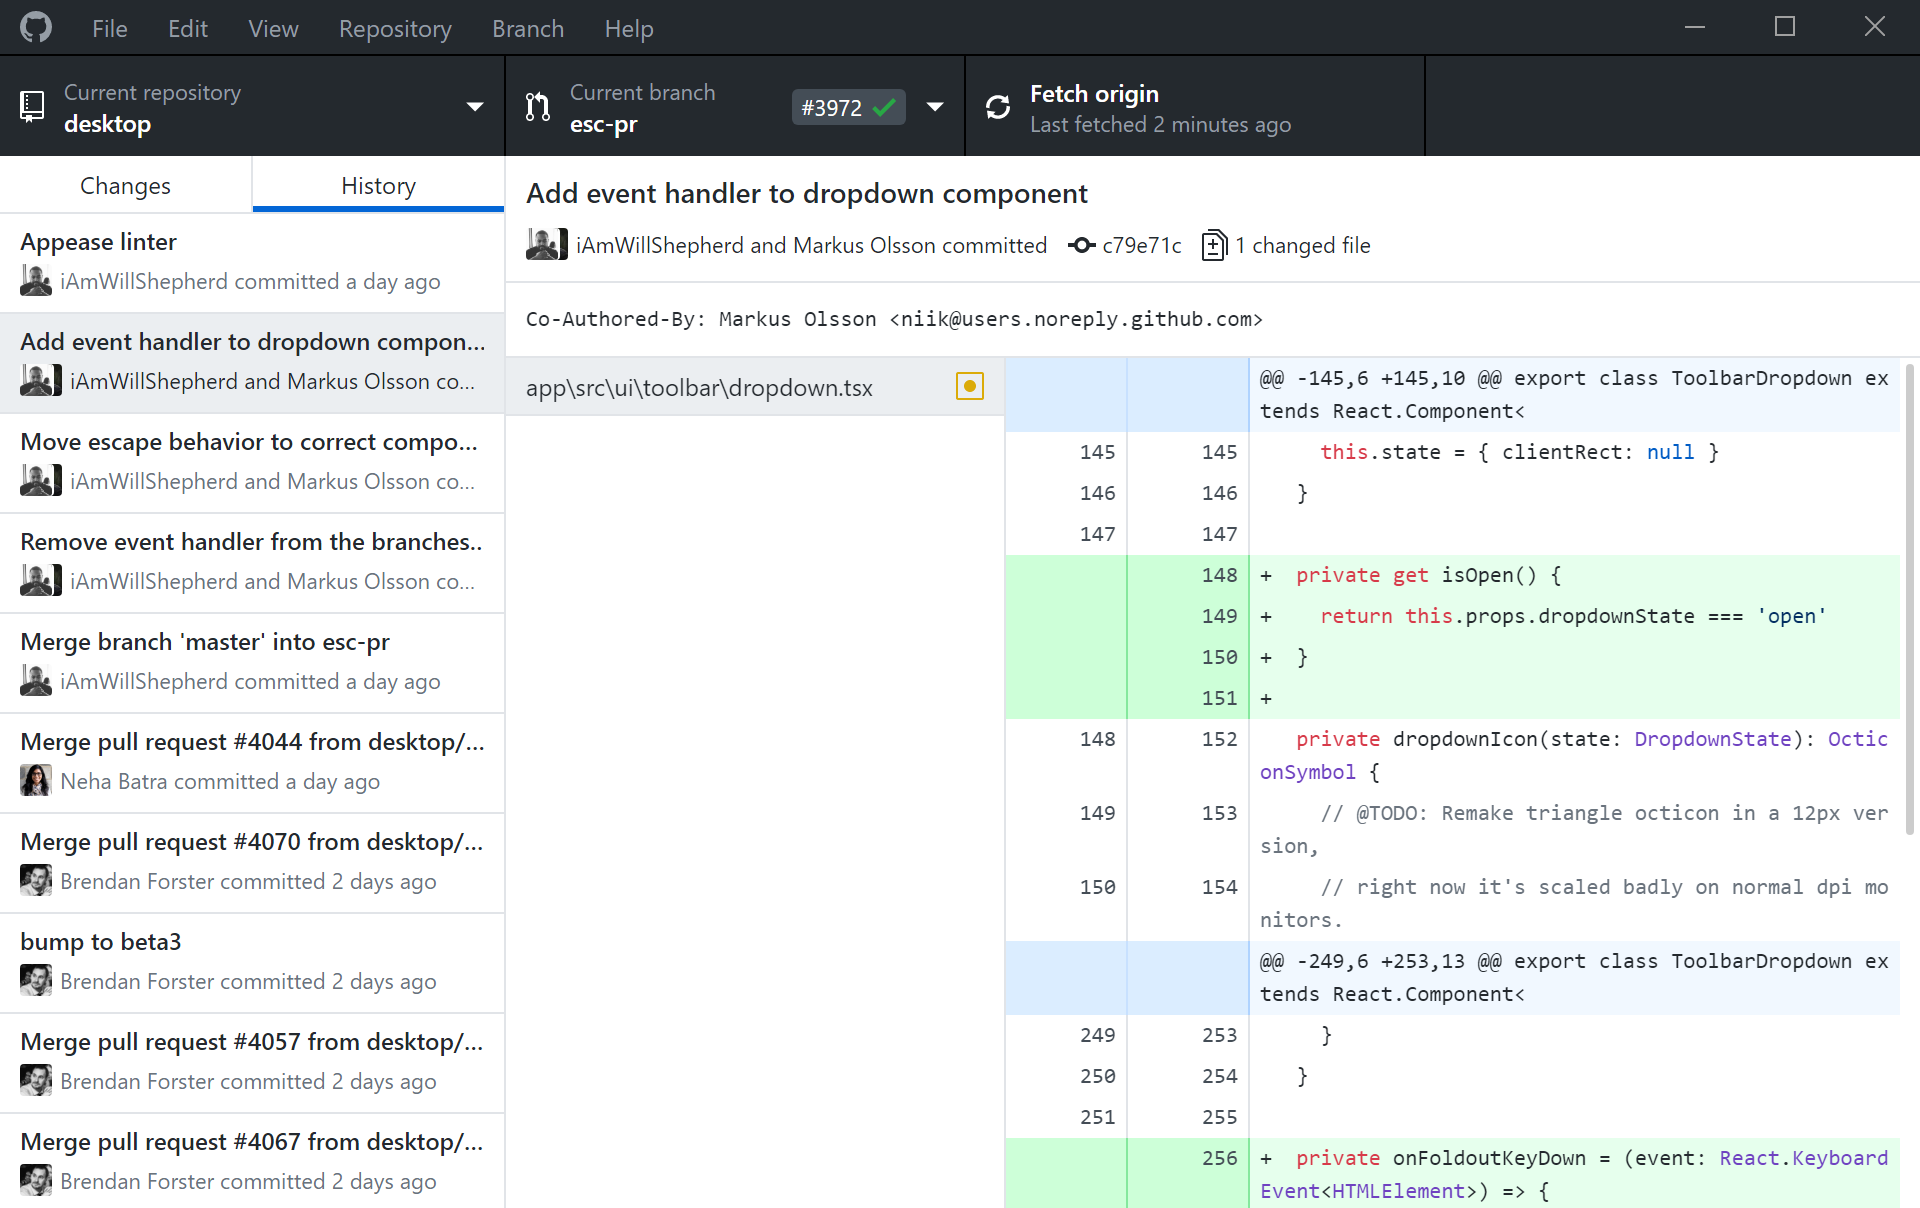
\includegraphics[scale=0.50]{github-desktop}
  \centering
  \caption{Github Desktop в Windows}
  \label{fig:github-desktop}
\end{figure}

